%% LyX 2.3.6.1 created this file.  For more info, see http://www.lyx.org/.
%% Do not edit unless you really know what you are doing.
\documentclass[english]{article}
\usepackage[T1]{fontenc}
\usepackage[latin9]{inputenc}
\usepackage{geometry}
\geometry{verbose,tmargin=2.5cm,bmargin=2.5cm,lmargin=2.5cm,rmargin=2.5cm}
\usepackage{graphicx}

\makeatletter

%%%%%%%%%%%%%%%%%%%%%%%%%%%%%% LyX specific LaTeX commands.
%% Because html converters don't know tabularnewline
\providecommand{\tabularnewline}{\\}

\makeatother

\usepackage{babel}
\begin{document}
{[}SPLIT\_HERE{]}
\begin{enumerate}
\item \textbf{{[}HCI/PRELIM/9597/2016/P1/Q1{]} }

A \textbf{\emph{palindrome}} is an integer that reads the same backwards
and forwards -- so 6, 11 and 121 are all palindromes, while 10, 12,
223 and 2244 are not (even though 010=10, we don't consider leading
zeroes when determining whether a number is a palindrome). 

A \textbf{\emph{fair and square}} number is an integer that is a \emph{palindrome}
\textbf{and} the \emph{square of a palindrome} at the same time. For
instance, 1, 9 and 121 are fair and square (being palindromes and
squares, respectively, of 1, 3 and 11), while 16, 22 and 676 are not
fair and square: 16 is \textbf{not} a palindrome, 22 is not a square,
and while 676 is a palindrome and a square number, it is the square
of 26, which is not a palindrome.

\subsection*{Task 1.1 }

Write program code with the following specification: 
\begin{itemize}
\item Input two integers -{}- the endpoints of an interval e.g. \texttt{100
1000 }
\item Output all fair and square numbers, if any, in the interval (inclusive
of endpoints). 
\item Output a count of the number of fair and square numbers in the interval.
\end{itemize}

\subsection*{Evidence 1: }

Your program code for Task 1.1.\hfill{} {[}8{]}

\subsection*{Evidence 2: }

Produce three screenshots showing the output of \texttt{1 4}, \texttt{10
120} and \texttt{100 1000} by the user.\hfill{} {[}3{]}

\subsection*{Task 1.2:}

Write program code to output the first 10 positive fair and square
numbers. 

\subsection*{Evidence 3: }

Your program code for Task 1.2.\hfill{} {[}3{]}

\subsection*{Evidence 4:}

Screenshot of output.\hfill{} {[}1{]}

{[}SPLIT\_HERE{]}
\item \textbf{{[}HCI/PRELIM/9597/2016/P1/Q2{]} }

The data file \texttt{FRUITS.txt} contains a list of fruit names. 

\subsection*{Task 2.1 }

Write program code to sort the fruit names in \texttt{FRUITS.txt}
in descending order using insertion sort. 

\subsection*{Evidence 5: }

Your program code for Task 2.1. \hfill{}{[}7{]}

\subsection*{Evidence 6: }

Screenshot of output. \hfill{}{[}1{]}

\subsection*{Task 2.2 }

Write program code to insert fruit names in \texttt{FRUITS.txt} to
a binary search tree using a linked structure.

\subsection*{Evidence 7:}

Your program code for Task 2.2. \hfill{}{[}8{]}

\subsection*{Task 2.3 }

Write program code to display the binary search tree contents in preorder,
inorder and postorder. 

\subsection*{Evidence 8: }

Your program code.\hfill{} {[}6{]}

\subsection*{Evidence 9: }

Screenshot of output.\hfill{} {[}3{]}

{[}SPLIT\_HERE{]}
\item \textbf{{[}HCI/PRELIM/9597/2016/P1/Q3{]} }

A transport company has a number of vehicles which can carry passengers.
Each vehicle is classified either as a bus or as a coach. All vehicles
have a registration number and have a certain number of seats for
the passengers. A bus can have a maximum number of standing passengers,
but a coach is not allowed to carry any standing passengers. Some
of the coaches are fitted with seat belts, but seat belts are never
fitted in a bus.

The transport company currently has a data file,\texttt{ VEHICLE.dat},
stores the following data:
\begin{itemize}
\item \texttt{RegNo} is used to uniquely identify a particular vehicle.
A typical vehicle registration number comes in the format \textquotedbl SBA1234\textquotedbl :
\begin{itemize}
\item S -- vehicle class (\textquotedbl S\textquotedbl{} stands for a
private vehicle) 
\item BA -- alphabetical series (\textquotedbl I\textquotedbl{} and \textquotedbl O\textquotedbl{}
are not used to avoid confusion with \textquotedbl 1\textquotedbl{}
and \textquotedbl 0\textquotedbl ) 
\item 1234 -- numerical series 
\end{itemize}
\item \texttt{NoOfSeats} is the maximum number of seats for passengers that
each vehicle can carry. 
\item \texttt{VehicleType} is the type of the vehicle and can take one of
the two values: \textquoteleft \texttt{B}\textquoteright{} for a bus
and \textquoteleft C\textquoteright{} for a coach. 
\end{itemize}
\texttt{VEHICLE.dat} has the following structure: 

\noindent %
\noindent\begin{minipage}[t]{1\columnwidth}%
\texttt{<NumberOfRecords>}

\texttt{<RegNo>|<NoOfSeats>|<VehicleType> }

\texttt{<RegNo>|<NoOfSeats>|<VehicleType> }

\texttt{. . . . . . . . . . . . . . . }

\texttt{. . . . . . . . . . . . . . . }

\texttt{<RegNo>|<NoOfSeats>|<VehicleType> }%
\end{minipage}

\texttt{NumberOfRecords} is the number of records in the file.

\subsection*{Task 3.1 }

Complete the test case table with the addition of \textbf{three} more
invalid vehicle registration numbers. The reasons for their invalidity
should be different.

The return value is a code as follows: 
\begin{itemize}
\item 0 -- valid registration number 
\item 1 -- the registration number was not 7 characters 
\item you will use other integer numbers for other invalid cases.

\begin{tabular}{|c|c|c|c|}
\hline 
Test Number & \texttt{RegNo} & Return value & Explanation of the test case\tabularnewline
\hline 
1 & \texttt{SBA1234} & \texttt{0} & Valid registration number\tabularnewline
\hline 
2 &  &  & \tabularnewline
\hline 
3 &  &  & \tabularnewline
\hline 
4 &  &  & \tabularnewline
\hline 
\end{tabular}
\end{itemize}

\subsection*{Evidence 10: }

The completed test case table. \hfill{}{[}3{]}

\subsection*{Task 3.2 }

Write program code for a function to validate a registration number.
The function header has the format:
\noindent \begin{center}
\texttt{FUNCTION ValidateRegNo(ThisRegNo : STRING) RETURNS INTEGER }
\par\end{center}

Write a program to:
\begin{itemize}
\item Input a registration number by the user 
\item Validate the input using the function \texttt{ValidateRegNo} 
\item Output a message describing the validity of the input.
\end{itemize}

\subsection*{Evidence 11:}
\begin{itemize}
\item Program code for the function \texttt{ValidateRegNo}\hfill{} {[}4{]}
\item Three screenshots showing the testing of Test Numbers 2, 3 and 4..
\hfill{}{[}3{]}
\end{itemize}
Additional data now needs to be stored about the vehicle:
\begin{itemize}
\item \texttt{MaxStanding} is the maximum number of standing passengers
that a vehicle classified as of type \textquoteleft \texttt{B}\textquoteright{}
can carry.
\item \texttt{SeatBeltsFitted} is a field that indicates whether a vehicle
of type \textquoteleft \texttt{C}\textquoteright{} has fitted with
seat belts.
\end{itemize}
The program design to process data about the vehicles is to be implemented
with objectoriented programming with the following three classes: 
\begin{center}
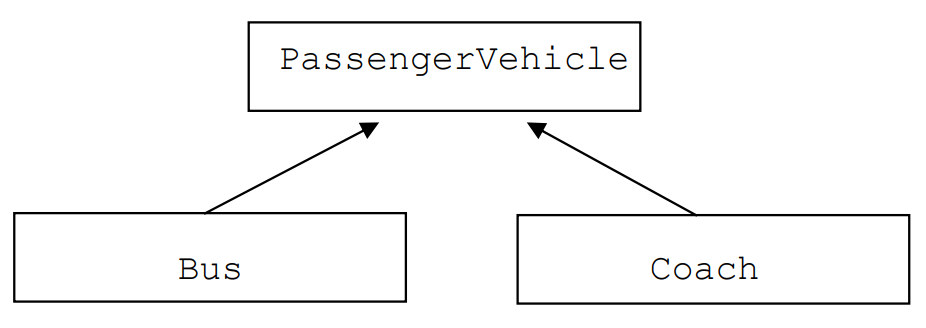
\includegraphics[width=0.35\paperwidth]{C:/Users/Admin/Desktop/Github/question_bank/LyX/static/img/9597-HCI-2016-P1-Q3-1}
\par\end{center}

\subsection*{Task 3.3 }

Write program code for the three classes shown. Evidence 12: Program
code for the three classes. \hfill{}{[}6{]}

\subsection*{Task 3.4 }

The data in \texttt{VEHICLE.dat} does not currently contain the following
additional data: 
\begin{itemize}
\item MaxStanding 
\item SeatBeltsFitted 
\end{itemize}
Write code to read a record from \texttt{VEHICLE.dat} and write the
updated record to \texttt{UVEHICLE.dat}.

As the data on each vehicle is read it should be displayed and the
user should be allowed to input the additional data required.

The user should be prompted to input the data item appropriate to
the type of vehicle.

The number of standing passengers is never more than 15.

For a \textquoteleft \texttt{C}\textquoteright{} type vehicle the
\texttt{MaxStanding} field should contain a zero value. 

The \texttt{SeatBeltsFitted} field should contain an appropriate value.
You are expected to make use of the classes you designed in Task 3.3.

\subsection*{Evidence 13: }

Program code for Task 3.4.\hfill{} {[}10{]}

\subsection*{Evidence 14: }

Screenshot showing the contents of \texttt{UVEHICLE.dat} from running
the program.\hfill{} {[}2{]}

{[}SPLIT\_HERE{]}
\item \textbf{{[}HCI/PRELIM/9597/2016/P1/Q4{]} }

A program is to be written to represent and implement a linked list
of nodes. Each node contains a string data value and a pointer. The
pointers link the data items in alphabetical order. 

The unused nodes are linked as shown below. The first unused node
is the position where the next new data item is to be stored. 
\begin{center}
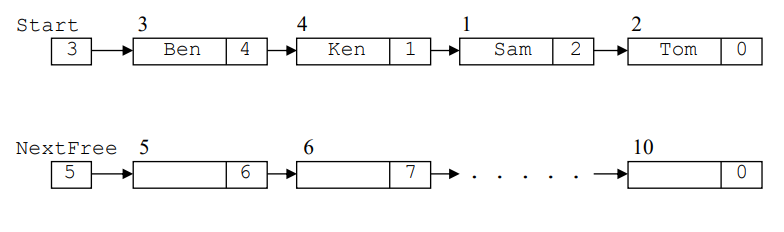
\includegraphics[width=0.65\paperwidth]{C:/Users/Admin/Desktop/Github/question_bank/LyX/static/img/9597-HCI-2016-P1-Q4-1}
\par\end{center}

The diagram shows the linked list with:
\begin{itemize}
\item the names \texttt{Sam}, \texttt{Tom}, \texttt{Ben} and \texttt{Ken}
(added in that order). 
\item the unused nodes linked together. 
\end{itemize}
The program will use a user-defined type \texttt{ListNode} for each
node defined as follows:
\noindent \begin{center}
\begin{tabular}{|c|c|c|}
\hline 
Identifier & Data Type & Description\tabularnewline
\hline 
\texttt{DataValue} & \texttt{STRING} & The node data\tabularnewline
\hline 
\texttt{PointerValue} & \texttt{INTEGER} & The node pointer \tabularnewline
\hline 
\end{tabular}
\par\end{center}

A linked list is implemented as an instance of the class \texttt{LinkedList}.
The class \texttt{LinkedList} has the following properties and methods:
\begin{center}
\begin{tabular}{|l|l|l|}
\hline 
\multicolumn{3}{|c|}{\texttt{Class: LinkedList}}\tabularnewline
\hline 
\multicolumn{3}{|c|}{Properties}\tabularnewline
\hline 
\texttt{\hspace{0.01\columnwidth}}Identifier & \texttt{\hspace{0.01\columnwidth}}Data Type & \texttt{\hspace{0.05\columnwidth}}Description\tabularnewline
\hline 
\texttt{Node} & \texttt{ARRAY{[}10{]} OF ListNode} & The linked list data structure -- data values and pointers. The array
index starts at 1. For testing purposes, the dataset has a maximum
of 10 items.\tabularnewline
\hline 
\texttt{Start} & \texttt{INTEGER} & Index position of the node at the start of the linked list. \tabularnewline
\hline 
\texttt{NextFree} & \texttt{INTEGER} & Index position of the next unused node.\tabularnewline
\hline 
\end{tabular}
\par\end{center}

\begin{center}
\begin{tabular}{|l|l|l|}
\hline 
\multicolumn{3}{|c|}{Methods}\tabularnewline
\hline 
\texttt{Initialise} & \texttt{PROCEDURE} & Sets all node data values to empty string. Set pointers to indicate
all nodes are unused and linked. Initialise values for \texttt{Start}
and \texttt{NextFree}.\tabularnewline
\hline 
\texttt{AddNode} & \texttt{PROCEDURE} & Add a new data item to the linked list. \tabularnewline
\hline 
\texttt{RemoveNode} & \texttt{PROCEDURE} & Remove a data item from the linked list.\tabularnewline
\hline 
\texttt{Display} & \texttt{PROCEDURE} & Display the current state of pointers and the array contents.\tabularnewline
\hline 
\texttt{IsEmpty} & \texttt{BOOLEAN FUNCTION} & Test for empty linked list. \tabularnewline
\hline 
\texttt{IsFull} & \texttt{BOOLEAN FUNCTION} & Test for no unused nodes.\tabularnewline
\hline 
\end{tabular}
\par\end{center}

\subsection*{Task 4.1 }

Write program code that repeatedly: 
\begin{itemize}
\item displays a menu with the following choices: 
\begin{enumerate}
\item[1.]  Add an item
\item[2.]  Remove an item 
\item[3.]  Output all pointers and data values 
\item[4.]  Exit 
\end{enumerate}
\item calls an appropriate procedure depending on the user\textquoteright s
choice. 
\end{itemize}

\subsection*{Evidence 15: }

Program code for Task 4.1. \hfill{}{[}5{]}

\subsection*{Task 4.2 }

Write program code for the classes \texttt{ListNode} and \texttt{LinkedList}.
Including the \texttt{Initialise}, \texttt{IsEmpty}, \texttt{IsFull}
and \texttt{Display} methods. The code should follow the specification
given. Do not attempt to write the methods \texttt{AddNode} and \texttt{RemoveNode}
at this stage.

\subsection*{Evidence 16: }

Program code for the \texttt{ListNode} and \texttt{LinkedList} classes
\hfill{}{[}10{]}

\subsection*{Task 4.3 }

Write code to create a \texttt{LinkedList} object in the main program. 

Run the program and select menu choice 3 to confirm the initial values
of the pointers and data values when the linked list is empty. 

\subsection*{Evidence 17:}

Screenshot confirming all values after initialisation of the \texttt{LinkedList}
object.\hfill{} {[}2{]}

Consider the \texttt{AddNode} method. The following pseudocode adds
a new data item to the linked list. The algorithm uses the variables
below:
\begin{center}
\begin{tabular}{|l|l|l|}
\hline 
\texttt{\hspace{0.01\columnwidth}}Identifier & \texttt{\hspace{0.01\columnwidth}}Data Type & \texttt{\hspace{0.05\columnwidth}}Description\tabularnewline
\hline 
NewItem & STRING & New data item input by the user\tabularnewline
\hline 
Found & BOOLEAN & lags to TRUE when the position at which to insert the new item has
been found\tabularnewline
\hline 
Current & INTEGER & array index position during list traversal\tabularnewline
\hline 
Previous & INTEGER & Previous array index position during list traversal\tabularnewline
\hline 
Temp & INTEGER & Temporary storage of pointer value\tabularnewline
\hline 
\end{tabular}
\par\end{center}

\noindent %
\noindent\begin{minipage}[t]{1\columnwidth}%
\texttt{PROCEDURE AddNode}

\texttt{\qquad{}INPUT NewItem}

\texttt{\qquad{}Node{[}NextFree{]}.DataValue = NewItem}

\texttt{\bigskip{}
}

\texttt{\qquad{}Temp = NextFree }

\texttt{\qquad{}NextFree = Node{[}NextFree{]}.PointerValue }

\texttt{\bigskip{}
}

\texttt{\qquad{}\# traverse the list to find the position to }

\texttt{\qquad{}\# insert the new item }

\texttt{\qquad{}Found = False }

\texttt{\qquad{}Current = Start }

\texttt{\qquad{}Previous = 0}

\texttt{\bigskip{}
}

\texttt{\qquad{}WHILE NOT Found AND Current != 0 }

\texttt{\qquad{}\qquad{}IF NewItem > Node{[}Current{]}.DataValue}

\texttt{\qquad{}\qquad{}\qquad{}THEN}

\texttt{\qquad{}\qquad{}\qquad{}\qquad{}\# move on to the next
node }

\texttt{\qquad{}\qquad{}\qquad{}\qquad{}Previous = Current }

\texttt{\qquad{}\qquad{}\qquad{}\qquad{}Current = Node{[}Current{]}.PointerValue}

\texttt{\qquad{}\qquad{}\qquad{}ELSE }

\texttt{\qquad{}\qquad{}\qquad{}\qquad{}Found = True }

\texttt{\qquad{}\qquad{}ENDIF}

\texttt{\qquad{}ENDWHILE}

\texttt{\bigskip{}
}

\texttt{\qquad{}IF Previous = 0 }

\texttt{\qquad{}\qquad{}THEN }

\texttt{\qquad{}\qquad{}\qquad{}\# new item will become the start
of the list}

\texttt{\qquad{}\qquad{}\qquad{}Start = Temp }

\texttt{\qquad{}\qquad{}\qquad{}Node{[}Temp{]}.PointerValue = Current }

\texttt{\qquad{}\qquad{}ELSE}

\texttt{\qquad{}\qquad{}\qquad{}\# new item is between previous
and current }

\texttt{\qquad{}\qquad{}Node{[}Previous{]}.PointerValue = Temp}

\texttt{\qquad{}\qquad{}Node{[}Temp{]}.PointerValue = Current }

\texttt{\qquad{}ENDIF }

\texttt{ENDPROCEDURE}%
\end{minipage}

Identifier Data Type Description F Current Note: The above pseudocode
is available in the text file \texttt{PSEUDOCODE\_TASK\_4\_4.txt}

\subsection*{Task 4.4 }

Write code to implement the \texttt{AddNode} method for the \texttt{LinkedList}
class. 

You may use the text file \texttt{PSEUDOCODE\_TASK\_4\_4.txt} as a
basis for the writing of your code.

The main program should check each time that the \texttt{LinkedList}
object is not full before using the \texttt{AddNode} method.

Run the program as follows: 
\begin{itemize}
\item Menu choice 1 four times, inputting the data values:

\texttt{Sam}, \texttt{Tom}, \texttt{Ben}, \texttt{Ken} in that order. 
\item Menu choice 3 to display.
\end{itemize}

\subsection*{Evidence 18: }

Your program code for Task 4.4. \hfill{}{[}5{]}

\subsection*{Evidence 19: }

Screenshot showing the pointers and the addition of the four nodes
to the linked list. \hfill{}{[}2{]}

\subsection*{Task 4.5 }

Write code to implement the \texttt{RemoveNode} method for the \texttt{LinkedList}
class. 

The main program should check each time that the LinkedList object
is not empty before using the \texttt{RemoveNode} method. Node removed
from the linked list should be returned to the NextFree list. 

Run the program as follows: 
\begin{itemize}
\item Menu choice 1 four times, inputting the data values: 

\texttt{Sam}, \texttt{Tom}, \texttt{Ben}, \texttt{Ken} in that order. 
\item Menu choice 2 two times, inputting the data values: 

\texttt{Sam}, \texttt{Ben} in that order.
\item Menu choice 3 to display. 
\end{itemize}

\subsection*{Evidence 20: }

Your program code for Task 4.5. \hfill{}{[}6{]}

\subsection*{Evidence 21: }

Screenshot showing the pointers and data values after the addition
of the four nodes followed by the removal of two nodes to the linked
list. \hfill{}{[}2{]}

{[}SPLIT\_HERE{]}
\item \textbf{{[}HCI/PRELIM/9597/2016/P2/Q1{]} }

Using the information in the table below, assuming that the project
team will work a standard working week (5 working days in 1 week)
and that all tasks will start as soon as possible: 
\noindent \begin{center}
\begin{tabular}{|c|l|c|c|}
\hline 
Task & Description & Duration (Working Days) & Predecessor/s \tabularnewline
\hline 
A & Requirement Analysis & 5 & -\tabularnewline
\hline 
B & Systems Design & 15 & A\tabularnewline
\hline 
C & Programming & 25 & B\tabularnewline
\hline 
D & Telecoms & 15 & B\tabularnewline
\hline 
E & Hardware Installation & 30 & B\tabularnewline
\hline 
F & Integration & 10 & C, D\tabularnewline
\hline 
G & System Testing & 10 & E, F\tabularnewline
\hline 
H & Training/Support & 5 & G\tabularnewline
\hline 
I & Handover and Go-Liv & 5 & H\tabularnewline
\hline 
\end{tabular}
\par\end{center}
\begin{enumerate}
\item Draw a Program Evaluation and Review Technique (PERT) chart, show
clearly the early start and late start time of each task, showing
dummy tasks, where necessary. \hfill{}{[}4{]}
\item Explain the nature and purpose of a dummy activity. \hfill{}{[}2{]}
\item Explain dependent stages and concurrent stages, giving examples from
your chart. \hfill{}{[}2{]}
\item State the critical path and the minimum time in which the project
can be completed in weeks.\hfill{} {[}2{]}
\item Identify any non-critical tasks and the float (free slack) on each.\hfill{}
{[}2{]}
\item Produce a Gantt chart based on the above information.\hfill{} {[}2{]}
\end{enumerate}
{[}SPLIT\_HERE{]}
\item \textbf{{[}HCI/PRELIM/9597/2016/P2/Q2{]} }

The owner of HC Book Caf� wishes to converts his book caf� into a
self-service book club caf� for members only. All access to food or
books is via a \textquotedblleft vending machine\textquotedblright{}
concept using the member\textquoteright s card. 

There is a stock of 2000 different book titles and multiple copies
of popular titles. Books may be hired by members. Different rates
are charged for different books. Members are allowed to hire no more
than 5 items at anytime. 

Members can enjoy a light snack while viewing their favourite book.
If the book is returned the same day via the book drop, hire charges
are not incurred. All food and hire charges incurred for the month
is billed to the member every 12th of the following month. Cash transaction
is not available. 

The shop owner wishes to computerize the system to handle the various
transactions and stock control. The system should also perform the
following functions: 
\begin{itemize}
\item Hold up-to-date details of members and stock
\item Allow enquiry to determine the whereabouts, and dates of return, of
particular books 
\item Produce an itemized bill for each customer at end of each month.
\end{itemize}
\begin{enumerate}
\item The system analyst of a software house was to design the computerized
system. What documentation should the system analyst produce and state
5 necessary contents of the documentation? Who would use it and state
2 reasons for use.\hfill{} {[}8{]}
\item List the files, giving details of the fields which it may contain,
that would be required for this system, and draw the data flow diagram
of the computerized system. \hfill{} {[}12{]}
\item HC Book Caf� offers a member loyalty program that offers a range of
discounts. For members in the loyalty program between 3 to 5 years,
they will receive a 5\% discount. For more than 5 years, the member
will receive a 10\% discount. However, whether a member is in the
loyalty program or not, if the cumulative value of his transactions
for this calendar year exceed \$1000, he will receive a 15\% discount.
However, note that aggregation of discounts is not allowed. 
\begin{enumerate}
\item Create a decision table that shows all possible outcomes for the above
loyalty program. 
\item Draw the decision table after redundancies have been removed. \hfill{}
{[}5{]}
\end{enumerate}
\end{enumerate}
{[}SPLIT\_HERE{]}
\item \textbf{{[}HCI/PRELIM/9597/2016/P2/Q3{]} }

Given two positive integers \texttt{M} and \texttt{N}, the function
\texttt{GCD(M, N)} is defined by 
\begin{enumerate}
\item[(i)]  If \texttt{M < N}, swap \texttt{M} and \texttt{N} 
\item[(ii)]  Divide \texttt{M} by \texttt{N} and let \texttt{R} be the remainder.
If \texttt{R = 0}, \texttt{N} is the answer 
\item[(iii)]  Set \texttt{M = N}, \texttt{N = R} and go back to step (i)
\end{enumerate}
Produce a recursive solution for \texttt{GCD(M,N)} using pseudocode.
You may assume the availability of the operator \texttt{MOD} as in
part \textbf{(b)}.\hfill{} {[}6{]}

{[}SPLIT\_HERE{]}
\item \textbf{{[}HCI/PRELIM/9597/2016/P2/Q4{]} }
\begin{enumerate}
\item Explain what is meant by ASCII code and Unicode.\hfill{} {[}4{]}
\item A number is stored as a one byte binary integer. How would the number
99 be represented as a one byte binary? \hfill{}{[}2{]}
\item Convert the number 99 into hexadecimal. \hfill{}{[}2{]}
\item Give two reasons why hexadecimal numbers are used in computing. \hfill{}{[}2{]}
\end{enumerate}
{[}SPLIT\_HERE{]}
\item \textbf{{[}HCI/PRELIM/9597/2016/P2/Q5{]} }
\begin{enumerate}
\item Using the 3 design principle you have learnt in class to assess the
interfaces between IOS and Android for mobile. Redraw and complete
the table with your points. You may draw user interfaces to illustrate
your point. \hfill{}{[}15{]}
\noindent \begin{center}
\begin{tabular}{|l|c|c|}
\hline 
Design Principals & IOS & Android\tabularnewline
\hline 
Principal 1 &  & \tabularnewline
\hline 
Principal 2 &  & \tabularnewline
\hline 
Principal 3  &  & \tabularnewline
\hline 
\end{tabular}
\par\end{center}
\item From the table above, draw a brief conclusion on the usability of
the above platforms.\hfill{} {[}3{]}
\end{enumerate}
{[}SPLIT\_HERE{]}
\item \textbf{{[}HCI/PRELIM/9597/2016/P2/Q6{]} }

A relational database is to be used by the Human Resource department
to recruit and register new students at the beginning of each year.
Four tables present in the database are STUDENT, SCHOOL, GRADES, REGISTRATION. 

A brief description of the tables are as follow: 
\begin{itemize}
\item STUDENT table stores the demographic information of students
\item SCHOOL table stores information of the school they are currently studying
\item GRADES table stores information of the subjects and grades of the
student in the previous year
\item REGISTRATION ties together all the relevant information of the students
from other tables and their registration details
\end{itemize}
\begin{enumerate}
\item Draw an E-R diagram to show the relationship between the four tables
that provides for a fully normalized database design. \hfill{} {[}6{]}

A table description can be expressed as: 

\texttt{Tablename{[}Attribute1, Attribute2, \dots .. {]} }

The primary key is indicated by underlining one or more attributes. 
\end{enumerate}
(b) Give a table description for all the tables. Ensure there are
at least 2 attributes in addition to the primary key.\hfill{} {[}12{]}

{[}SPLIT\_HERE{]}
\item \textbf{{[}HCI/PRELIM/9597/2016/P2/Q7{]} }

Cloud computing is widely used in education to facilitate teaching
and learning in classrooms. 
\begin{enumerate}
\item How is computing from the Cloud different from computing traditionally?
\hfill{}{[}2{]}
\item What are the benefits of cloud computing?\hfill{} {[}4{]}
\item How can Cloud computing assist you as a student in project management?
\hfill{}{[}3{]}
\end{enumerate}
{[}SPLIT\_HERE{]}
\end{enumerate}

\end{document}
